%%%%%%%%%%%%%%%%%%%%%%%%%%%%%%%%%%%%%%%%%
% Beamer Presentation
% LaTeX Template
% Version 1.0 (10/11/12)
%
% This template has been downloaded from:
% http://www.LaTeXTemplates.com
%
% License:
% CC BY-NC-SA 3.0 (http://creativecommons.org/licenses/by-nc-sa/3.0/)
%
%%%%%%%%%%%%%%%%%%%%%%%%%%%%%%%%%%%%%%%%%

%----------------------------------------------------------------------------------------
%	PACKAGES AND THEMES
%----------------------------------------------------------------------------------------

\documentclass{beamer}
\mode<presentation> {

% The Beamer class comes with a number of default slide themes
% which change the colors and layouts of slides. Below this is a list
% of all the themes, uncomment each in turn to see what they look like.

%\usetheme{default}
%\usetheme{AnnArbor}
%\usetheme{Antibes}
%\usetheme{Bergen}
%\usetheme{Berkeley}
%\usetheme{Berlin}
%\usetheme{Boadilla}
%\usetheme{CambridgeUS}
%\usetheme{Copenhagen}
%\usetheme{Darmstadt}
%\usetheme{Dresden}
%\usetheme{Frankfurt}
%\usetheme{Goettingen}
%\usetheme{Hannover}
%\usetheme{Ilmenau}
%\usetheme{JuanLesPins}
%\usetheme{Luebeck}
\usetheme{Madrid}
%\usetheme{Malmoe}
%\usetheme{Marburg}
%\usetheme{Montpellier}
%\usetheme{PaloAlto}
%\usetheme{Pittsburgh}
%\usetheme{Rochester}
%\usetheme{Singapore}
%\usetheme{Szeged}
%\usetheme{Warsaw}

% As well as themes, the Beamer class has a number of color themes
% for any slide theme. Uncomment each of these in turn to see how it
% changes the colors of your current slide theme.

%\usecolortheme{albatross}
%\usecolortheme{beaver}
%\usecolortheme{beetle}
%\usecolortheme{crane}
%\usecolortheme{dolphin}
%\usecolortheme{dove}
%\usecolortheme{fly}
%\usecolortheme{lily}
%\usecolortheme{orchid}
%\usecolortheme{rose}
%\usecolortheme{seagull}
%\usecolortheme{seahorse}
%\usecolortheme{whale}
\usecolortheme{wolverine}

%\setbeamertemplate{footline} % To remove the footer line in all slides uncomment this line
%\setbeamertemplate{footline}[page number] % To replace the footer line in all slides with a simple slide count uncomment this line
%\setbeamertemplate{navigation symbols}{} % To remove the navigation symbols from the bottom of all slides uncomment this line
}

\usepackage{tabularx}
\usepackage{graphicx} % Allows including images
\usepackage{booktabs} % Allows the use of \toprule, \midrule and \bottomrule in tables

%----------------------------------------------------------------------------------------
%	TITLE PAGE
%----------------------------------------------------------------------------------------

\title[Newtons Backward Difference]{Finding f(x) Using Newtons Dackward Difference Table} % The short title appears at the bottom of every slide, the full title is only on the title page
\author{GROUP PRESENTATION\\(Group 9)} % Your name
\institute[] % Your institution as it will appear on the bottom of every slide, may be shorthand to save space
{\textbf{TEAM MEMBERS} \\ % Your institution for the title page
\textit{Nishitha Singh\\
Akanksha Panda\\
Geetha Sruthi Rudrapati\\
Harsimar Preet Kaur\\
Soumyodeep Nayak\\
Mayank Dey} % Your email address
}
\date{\today} % Date, can be changed to a custom date

\begin{document}

\begin{frame}
\titlepage % Print the title page as the first slide
\end{frame}

\begin{frame}
\frametitle{Contents} % Table of contents slide, comment this block out to remove it
\tableofcontents % Throughout your presentation, if you choose to use \section{} and \subsection{} commands, these will automatically be printed on this slide as an overview of your presentation
\end{frame}

%----------------------------------------------------------------------------------------
%	PRESENTATION SLIDES
%----------------------------------------------------------------------------------------

%------------------------------------------------
\section{Introduction} % Sections can be created in order to organize your presentation into discrete blocks, all sections and subsections are automatically printed in the table of contents as an overview of the talk
%------------------------------------------------

\subsection{About Backward Difference Method} % A subsection can be created just before a set of slides with a common theme to further break down your presentation into chunks

\begin{frame}

\frametitle{Backward Difference}

\begin{block}{Definition}

The differences $y_1–y_0, y_2–y_1$, $\cdot\cdot\cdot$ , $y_n–y_{n –1}$ when denoted by $\nabla y_1$, $\nabla y_2$, $\cdot\cdot\cdot$ , $\nabla y_n$, respectively, are called first backward difference. Thus, the first backward differences are $\nabla y_{r}$ = $y_{r}$ - $y_{r - 1}$. This formula is useful when the value of f(x) is required near the end of the table. h is called
the interval of difference and $u = \dfrac{x-x_{n}}{h}$, Here $a_n$ is last term.

\end{block}

Newton's backward difference is a method for approximating the derivative of a function at a specific point using a finite difference approach. It is used to calculate the value of the derivative at a specific point by using the function values at the previous points. This formula is called the "backward" difference formula because it uses function values from previous points in the backward direction. 

\end{frame}

%------------------------------------------------
\subsection{Backward Difference Table} % A subsection can be created just before a set of slides with a common theme to further break down your presentation into chunks

\begin{frame}

\frametitle{Backward Difference Table}
\begin{center}
\graphicspath{ {./pics/} }
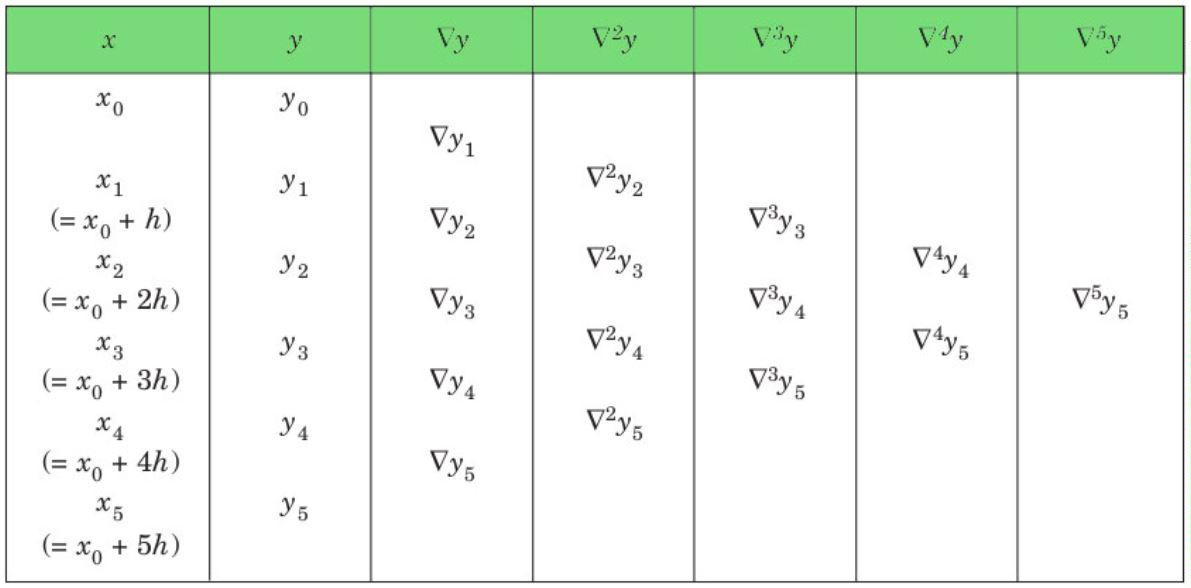
\includegraphics[width=12cm, height=7cm]{latexImage_1b5b126b0fa71b41c779e83b060d4927}
\end{center}
\end{frame}

%------------------------------------------------

\section{Solved Problems}
%------------------------------------------------
\subsection{Problem 1}
\begin{frame}
\frametitle{Solved Problem No. 1}
\begin{block}{Question}
The table gives the distance in nautical miles of the visible horizon for the given heights in feet above the earth’s surface:
\begin{table}
\centering
\begin{tabular}{|l|l|l|l|l|l|l|l|} 
\hline
x= height:    & 150   & 100   & 200   & 250   & 300   & 350   & 400    \\ 
\hline
y = distance: & 13.03 & 10.63 & 15.04 & 16.81 & 18.42 & 19.90 & 21.27  \\
\hline
\end{tabular}
\end{table}
Find the values of y when:\\
x = 410.
\end{block}
\end{frame}
\begin{frame}
\frametitle{Solution}
\begin{table}
Backward Difference Table\\\\
\centering
\begin{tabular}{|l|l|l|l|l|l|} 
\hline
\textbf{x}     & \textbf{y}       &\textbf{$\Delta$}       & \textbf{$\Delta^2$}      & \textbf{$\Delta^3$}     & \textbf{$\Delta^4$}       \\ 
\hline
$100$ & $10.63$ &        &         &        &          \\ 
\hline
      &         & $2.4$  &         &        &          \\ 
\hline
$150$ & $13.3$  &        & $-0.39$ &        &          \\ 
\hline
      &         & $2.01$ &         & $0.15$ &          \\ 
\hline
$200$ & $15.04$ &        & $-0.24$ &        & $-0.07$  \\ 
\hline
      &         & $1.77$ &         & $0.08$ &          \\ 
\hline
$250$ & $16.81$ &        & $-0.16$ &        & $-0.05$  \\ 
\hline
      &         & $1.61$ &         & $0.03$ &          \\ 
\hline
$300$ & $18.42$ &        & $-0.13$ &        & $-0.01$  \\ 
\hline
      &         & $1.48$ &         & $0.02$ &          \\ 
\hline
$350$ & $19.9$  &        & $-0.11$ &        &          \\ 
\hline
      &         & $1.37$ &         &        &          \\ 
\hline
$400$ & $21.27$ &        &         &        &          \\
\hline
\end{tabular}
\end{table}
\end{frame}
\begin{frame}
Since $x=410$ is near the end of the table, we use Newton's backward interpolation formula.

$$
\therefore \quad \text { Taking } x_{n}=400, p=\frac{x-x_{n}}{h}=\frac{10}{50}=0.2
$$

Using the line of backward difference

$$
y_{n}=21.27, \nabla y_{n}=1.37, \nabla^{2} y_{n}=-0.11, \nabla^{3} y_{n}=0.02 \text { etc. }
$$

$\therefore$ Newton's backward formula gives
$$
\begin{aligned}
& y_{410}=y_{400}+p \nabla y_{400}+\frac{p(p+1)}{2 !} \nabla^{2} y_{400} \\
& +\frac{p(p+1)(p+2)}{3 !} \Delta^{3} y_{400}+\frac{p(p+1)(p+2)(p+3)}{4 !} \nabla^{4} y_{400}+\cdots \\
& =21.27+0.2(1.37)+\frac{0.2(1.2)}{2 !}(-0.11) \\
& +\frac{0.2(1.2)(2.2)}{3 !}(0.02)+\frac{0.2(1.2)(2.2)(3.2)}{4 !}(-0.01) \\
& =21.27+0.274-0.0132+0.0018-0.0007 =21.53 \text { nautical miles }
\end{aligned}
$$
\end{frame}

%------------------------------------------------
\subsection{Problem 2}
\begin{frame}
\frametitle{Solved Problem No. 2}
\begin{block}{Question}
Find the cubic polynomial which takes the following values:
\begin{center}
\begin{tabular}{|c|c|c|c|c|}
\hline
$x:$ & 0 & 1 & 2 & 3 \\
\hline
$f(x):$ & 1 & 2 & 1 & 10 \\
\hline
\end{tabular}
\end{center}
Hence or otherwise evaluate $f(4)$.
\end{block}
\end{frame}

\begin{frame}{Solution}
The difference table is

\begin{center}
\begin{tabular}{|c|c|c|c|c|}
\hline
$x$ & $f(x)$ & $\Delta f(x)$ & $\Delta^{2} f(x)$ & $\Delta^{3} f(x)$ \\
\hline
0 & $\mathbf{1}$ &  &  &  \\
\hline
 &  & $\mathbf{1}$ &  &  \\
\hline
1 & 2 &  & $-\mathbf{2}$ &  \\
\hline
 &  & -1 &  & $\mathbf{1 2}$ \\
\hline
2 & 1 &  & $\mathbf{1 0}$ &  \\
\hline
 &  & $\mathbf{9}$ &  &  \\
\hline
3 & $\mathbf{1 0}$ &  &  &  \\
\hline
\end{tabular}
\end{center}
 Using Newton's backward interpolation formula, we get

$$
\begin{aligned}
f(4) & =f(3)+p \nabla f(3)+\frac{p(p+1)}{1.2} \nabla^{2} f(3)+\frac{p(p+1)(p+2)}{1.2 .3} \nabla^{3} f(3) \\
& =10+9+10+12=41
\end{aligned}
$$
\end{frame}
%------------------------------------------------
\section{Practice Problems}
%------------------------------------------------
\begin{frame}
\frametitle{Practice Problems}
\begin{block}{Problem 1}
Find the value of f(0.456) for the below given Newtons Backward Difference Table:
\begin{center}
\begin{tabular}{|c|c|c|c|c|}
\hline
$x$ & $y$ & $\Delta y$ & $\Delta^{2} y$ & $\Delta^{3} y$ \\
\hline
0.45 & 0.475482 &  &  &  \\
\hline
 &  & 0.009174 &  &  \\
\hline
0.46 & 0.484656 &  & 0.003622 &  \\
\hline
 &  & 0.012796 &  & -0.011120 \\
\hline 
0.47 & 0.497452 &  & -0.007498 &  \\
\hline
 &  & 0.005298 &  & 0.011118 \\
\hline
0.48 & 0.502750 &  & 0.003620 &  \\
\hline
&  & 0.008918 &  &  \\
\hline 
0.49 & 0.511668 &  &  &  \\
\hline
\end{tabular}
\end{center}
\end{block}
\end{frame}
\begin{frame}{}

\begin{block}{Problem 2}
Use Newton's backward interpolation formula to determine the value of $f(0.48)$ using the following table:

\begin{tabular}{|c|c|c|c|c|c|c|}
\hline
$x$ &  0.25 & 0.30 & 0.35 & 0.40 & 0.45 & 0.50 \\
\hline
$f(x)$ & 2.6754 & 2.8765 & 2.9076 & 3.2876 & 3.3451 & 3.7139 \\
\hline
\end{tabular}
\end{block}

\begin{block}{Problem 3}
The following table gives the value of $x$ and $y$.

\begin{center}
\begin{tabular}{|c|c|c|c|c|c|}
\hline
$x$ & 2 & 3 & 4 & 5 & 6 \\
\hline
$f(x)$ & 5 & 8 & 12 & 20 & 37 \\
\hline
\end{tabular}
\end{center}

Calculate the value of $y$ at $x=5.5$ by considering third degree Newton's backward interpolation polynomial. Again, find the same value by considering the fourth degree polynomial.
\end{block}
\end{frame}
\begin{frame}{}
\begin{block}{Problem 4}
The upward velocity of a rocket is given below:

\begin{center}
\begin{tabular}{|c|c|c|c|c|c|c|}
\hline
$t(\mathrm{sec})$ & 0 & 10 & 15 & 20 & 25 & 30 \\
$v(t)(\mathrm{m} / \mathrm{sec})$ & 0 & 126.75 & 350.50 & 510.80 & 650.40 & 920.25 \\
\hline
\end{tabular}
\end{center}
Determine the value of the velocity at $t=26 \mathrm{sec}$ using Newton's backward formulae.
\end{block}
\begin{block}{Problem 5}
Using Newton's backward difference formula, construct an interpolating polynomial of degree 3 for the data: $f(-0.75)=-0.0718125, f(-0.5)$ $=-0.02475, f(-0.25)=0.3349375, f(0)=1.10100$. Hence find $f(-1 / 3)$.
\end{block}
\end{frame}
%------------------------------------------------
\section{Practice Problem Solutions}
%------------------------------------------------
\subsection{Problem 1}
\begin{frame}
\frametitle{Solution for Problem 1}
For this problem, $x_{0}=0.45, x=0.456, h=0.01, u=\frac{x-x_{0}}{h}=\frac{0.456-0.45}{0.01}=0.6$. Now

$$
\begin{aligned}
y(0.456)= & y_{0}+u \Delta y_{0}+\frac{u(u-1)}{2 !} \Delta^{2} y_{0}+\frac{u(u-1)(u-2)}{3 !} \Delta^{3} y_{0} \\
= & 0.475482+0.6 \times 0.009174+\frac{0.6(0.6-1)}{2} \times 0.003622 \\
& +\frac{0.6(0.6-1)(0.6-2)}{6} \times(-0.011120) \\
= & 0.475482+0.0055044-0.0008693-0.0006227 \\
= & 0.4794944 .
\end{aligned}
$$

Hence, the value of $y$ when $x=0.456$ is 0.479494 .
\end{frame}
%------------------------------------------------
\subsection{Problem 2}
\begin{frame}
\frametitle{Solution for Problem 2}
 The backward difference table is

\begin{center}
\begin{tabular}{|c|c|c|c|c|c|}
\hline
$x$ & $f(x)$ & $\nabla f(x)$ & $\nabla^{2} f(x)$ & $\nabla^{3} f(x)$ & $\nabla^{4} f(x)$ \\
\hline
0.25 & 2.6754 &  &  &  &  \\
\hline
0.30 & 2.8765 & 0.2011 &  &  &  \\
\hline
0.35 & 2.9076 & 0.0311 & -0.1700 &  &  \\
\hline
0.40 & 3.2876 & 0.3800 & 0.3489 & 0.5189 &  \\
\hline
0.45 & 3.3451 & 0.0575 & -0.3225 & -0.6714 & -1.1903 \\
\hline
0.50 & 3.7139 & 0.3688 & 0.3113 & 0.6338 & 1.3052 \\
\hline
\end{tabular}
\end{center}

In this problem, $x_{n}=0.50, x=0.48, h=0.05, v=\frac{x-x_{n}}{h}=\frac{0.48-0.50}{0.05}=-0.4$. Then,

$$
\begin{aligned}
f(0.48)= & f\left(x_{n}\right)+v \nabla f\left(x_{n}\right)+\frac{v(v+1)}{2 !} \nabla^{2} f\left(x_{n}\right)+\frac{v(v+1)(v+2)}{3 !} \nabla^{3} f\left(x_{n}\right) \\
& +\frac{v(v+1)(v+2)(v+3)}{4 !} \nabla^{4} f\left(x_{n}\right)+\cdots \\
\end{aligned}
$$
\end{frame}

\begin{frame}
$$
\begin{aligned}
= & 3.7139-0.4 \times 0.3688+\frac{-0.4(-0.4+1)}{2} \times 0.3113 \\
& +\frac{-0.4(-0.4+1)(-0.4+2)}{6} \times 0.6338 \\
& +\frac{-0.4(-0.4+1)(-0.4+2)(-0.4+3)}{24} \times 1.3052 \\
= & 3.7139-0.14752-0.037356-0.040563-0.054296 \\
= & 3.43416 \simeq 3.4342 .
\end{aligned}
$$
Thus, $f(0.48)=3.4342$
\end{frame}
%------------------------------------------------
\subsection{Problem 3}
\begin{frame}
\frametitle{Solution for Problem 3}
To find a third degree polynomial, we consider last four data and the corresponding backward difference table is

\begin{center}
\begin{tabular}{|c|c|c|c|c|}
\hline
$x$ & $y$ & $\nabla y$ & $\nabla^{2} y$ & $\nabla^{3} y$ \\
\hline
3 & 8 &  &  &  \\
\hline
4 & 12 & 4 &  &  \\
\hline
5 & 20 & 8 & 4 &  \\
\hline
6 & 37 & 17 & 9 & 5 \\
\hline
\end{tabular}
\end{center}

In this problem, $x_{n}=6, x=5.5, h=1, v=\frac{x-x_{n}}{h}=\frac{5.5-6}{1}=-0.5$.

$$
\begin{aligned}
y(5.5)= & y_{n}+v \nabla y_{n}+\frac{v(v+1)}{2 !} \nabla^{2} y_{n}+\frac{v(v+1)(v+2)}{3 !} \nabla^{3} y_{n} \\
= & 37-0.5 \times 17+\frac{-0.5(-0.5+1)}{2} \times 9 \\
& +\frac{-0.5(-0.5+1)(-0.5+2)}{6} \times 5 \\
= & 37-8.5-1.125-0.3125 
= 27.0625 .
\end{aligned}
$$
\end{frame}
\begin{frame}{}
    
Now, we consider fourth degree polynomial to calculate $y(5.5)$. The difference table is shown below.

\begin{center}
\begin{tabular}{|c|c|c|c|c|c|}
\hline
$x$ & $y$ & $\nabla y$ & $\nabla^{2} y$ & $\nabla^{3} y$ & $\nabla^{4} y$ \\
\hline
2 & 5 &  &  &  &  \\
\hline
3 & 8 & 3 &  &  &  \\
\hline
4 & 12 & 4 & 1 &  &  \\
\hline
5 & 20 & 8 & 4 & 3 &  \\
\hline
6 & 37 & 17 & 9 & 5 & 2 \\
\hline
\end{tabular}
\end{center}
The value of $y(5.5)$ can be determined by the following formula. Note that there is only one term we have to calculate, other terms are already determined in previous step.\\
& $f(0.48)=y_{n}+v \nabla y_{n}+\frac{v(v+1)}{2 !} \nabla^{2} y_{n}+\frac{v(v+1)(v+2)}{3 !} \nabla^{3} y_{n}+\frac{v(v+1)(v+2)(v+3)}{4 !} \nabla^{4} y_{n}$.\\
The value of the last term is
$$
\begin{aligned}
\frac{v(v+1)(v+2)(v+3)}{4 !} \nabla^{4} y_{n} 
=\frac{-0.5(-0.5+1)(-0.5+2)(-0.5+3)}{4 !} \times 2\\
\textbf{=-0.078125.}
\end{aligned}
$$
\end{frame}
%------------------------------------------------
\subsection{Problem 4}
\begin{frame}
\frametitle{Solution for Problem 4}
The velocity at $t=0$ is zero, and hence it does not give any information. Therefore, we discard this data.

Using Newton's backward formula

The backward difference table is

\begin{center}
\begin{tabular}{|c|c|c|c|c|c|}
\hline
$t$ & $v(t)$ & $\nabla v$ & $\nabla^{2} v$ & $\nabla^{3} v$ & $\nabla^{4} v$ \\
\hline
10 & 126.75 &  &  &  &  \\
\hline
15 & 350.50 & 223.75 &  &  &  \\
\hline
20 & 510.80 & 160.30 & -63.45 &  &  \\
\hline
25 & 650.40 & 139.60 & -20.70 & 42.45 &  \\
\hline
30 & 920.25 & 269.85 & 130.25 & 150.95 & 108.50 \\
\hline
\end{tabular}
\end{center}

Here, $t_{n}=30, t=26, h=5, v=\frac{t-t_{n}}{h}=\frac{26-30}{5}=-0.8$.
\end{frame}
\begin{frame}{}
    
By Newton's backward formula

$$
\begin{aligned}
v(26)= & y_{n}+v \nabla y_{n}+\frac{v(v+1)}{2 !} \nabla^{2} y_{n}+\frac{v(v+1)(v+2)}{3 !} \nabla^{3} y_{n} \\
& +\frac{v(v+1)(v+2)(v+3)}{4 !} \nabla^{4} y_{n} \\
= & 920.25-0.8 \times 269.85+\frac{-0.8(-0.8+1)}{2} \times(130.25) \\
& +\frac{-0.8(-0.8+1)(-0.8+2)}{6} \times 150.95 \\
& +\frac{-0.8(-0.8+1)(-0.8+2)(-0.8+3)}{24} \times 108.50 \\
= & 687.21 .
\end{aligned}
$$

Thus the velocity of the rocket at $t=16 \mathrm{sec}$ is $687.21 \mathrm{~m} / \mathrm{s}$.
\end{frame}
%------------------------------------------------
\subsection{Problem 5}
\begin{frame}
\frametitle{Solution for Problem 5}
The difference table is

\begin{center}
\begin{tabular}{|c|c|c|c|c|}
\hline
$x$ & $y$ & $\Delta y$ & $\Delta^{2} y$ & $\Delta^{3} y$ \\
\hline
-0.75 & -0.0718125 &  &  &  \\
\hline
 &  & 0.0470625 &  &  \\
\hline
-0.50 & -0.02475 &  & 0.312625 &  \\
\hline
 &  & 0.3596875 &  & $\mathbf{0 . 0 9 3 7 5}$ \\
\hline
-0.25 & 0.3349375 &  & $\mathbf{0 . 4 0 0 3 7 5}$ &  \\
\hline
 &  & $\mathbf{0 . 7 6 6 0 6 2 5}$ &  &  \\
\hline
$\mathbf{0}$ & $\mathbf{1 . 1 0 1 0 0}$ &  &  &  \\
\hline
\end{tabular}
\end{center}
\end{frame}
\begin{frame}{}
We use Newton's backward difference formula

$$
\begin{aligned}
y(x) & =y_{3}+\frac{p}{1 !} \nabla y_{3}+\frac{p(p+1)}{2 !} \nabla^{2} y_{3}+\frac{p(p+1)(p+2)}{3 !} \nabla^{3} y_{3} \\
\text { taking } \quad x_{3} & =0, p=\frac{x-0}{h}=\frac{x}{0.25}=4 x \quad[\because h=0.25]
\end{aligned}
$$

$$
\begin{aligned}
y(x)= & 1.10100+4 x(0.7660625)+\frac{4 x(4 x+1)}{2}(0.400375) \\
& +\frac{4 x(4 x+1)(4 x+2)}{6}(0.09375) \\
& =1.101+3.06425 x+3.251 x^{2}+0.81275 x+x^{3}+0.75 x^{2}+0.125 x \\
& =x^{3}+4.001 x^{2}+4.002 x+1.101
\end{aligned}
$$

Put $\quad x=-\frac{1}{3}$, so that

$$
\begin{aligned}
y\left(-\frac{1}{3}\right) & =\left(-\frac{1}{3}\right)^{3}+4.001\left(-\frac{1}{3}\right)^{2}+4.002\left(-\frac{1}{3}\right)+1.101 = 0.1745
\end{aligned}
$$
\end{frame}
%------------------------------------------------
\begin{frame}
\begin{center}
{\fontsize{40}{50}\selectfont Thank You for your Patience!!!!}
\end{center}
\end{frame}
%-------------------------------------------------------------------------------------
\end{document}